
\documentclass[
12pt,
a4paper,
bibliography=totocnumbered, %Literaturverzereichnis als Eintrag ins Inhaltsverzeichnis
%twoside, %Zweiseitiger Druck
BCOR=1cm, %Platz zum Lochen
oneside, %Einseitiger Druck
]{scrartcl}

\usepackage{geometry}

\usepackage[default]{fontsetup}
%\usepackage[onehalfspacing]{setspace}

\usepackage[ngerman]{babel}
\usepackage[babel=true,german=quotes]{csquotes}

\usepackage{microtype}
\usepackage{mleftright}
%\newcommand{\Le}{\mleft}
%\newcommand{\Ri}{\mright}
\usepackage[no-script, no-scriptscript, no-inner, no-close]{innerscript}

% Mathepakete (unicode-math ersetzt amssymb, amsfonts etc.)
\usepackage{amsmath,amsthm}
\usepackage{mathtools}
\usepackage{fixdif,derivative}
\usepackage{physics2}
\usephysicsmodule{ab.legacy}

\usepackage{unicode-math}
\setmathfont{NewCMMath-Book}
\setmathfont{NewCMMath-Book}[range=cal, StylisticSet=1]
\setmathfont{NewCMMath-Book}[range=scr]

\usepackage{siunitx}
\sisetup{detect-weight=true, detect-family=true,locale=DE,range-phrase={\,bis\,},list-final-separator ={\,\linebreak[0] \text{und}\,},separate-uncertainty=true,per-mode = symbol-or-fraction}
%\SI[per-mode = fraction]{1}{\meter\per\second} erzwingt auch im Fließtext die Bruchdarstellung.
\DeclareSIUnit\curie{Ci}%Zusätzliche Einheit definieren

\usepackage{tabularx, booktabs, multirow}
\usepackage{array}
\usepackage{enumitem}
\usepackage{float}
\usepackage{graphicx}
\usepackage{xurl}

\usepackage[final]{pdfpages}
\usepackage{framed, color} %Framed: Paket, mittels dessen ein Rahmen um einen Bereich definiert werden kann. Color: Lässt Farbdarstellung in Schrift, Hintergrund etc. zu

\usepackage{scrlayer-scrpage} %Header für die KOMA-script-Klasse

%\usepackage[square,numbers]{natbib}
\usepackage{subfigure} %Mehrere Bilder in einer Figure-Umgebung

\usepackage[bookmarks,colorlinks=true]{hyperref}
\hypersetup{
	colorlinks,
	linktocpage,
	citecolor=black,
	filecolor=black,
	linkcolor=black,
	urlcolor=black,
	pdftitle=X,
	pdfauthor=JM-VS
}

\usepackage[backend=biber, style=chem-angew]{biblatex}
\addbibresource{lit.bib}

\numberwithin{equation}{section} % Die Nummerierung von Gleichungen bekommt die jeweilige Section-Nummer als Präfix

\setlength{\parindent}{0pt} %Einrücktiefe von neuen Absätzen
\setlength{\parskip}{6pt} %Abstand von Absätzen

\pagestyle{scrheadings}%Kopf und Fußzeilen
\ohead{\textbf{\GRUPPENNR\ - \VERSUCHSNR}} %Header oben links auf linker Seite (ungerade Seitenzahl) und oben rechts auf rechter Seite (gerade Seitenzahl), beinhaltet gruppennummer und Versuchskürzel. Im Fall eine einseitigen Dokuments: Header oben rechts
\ihead{\VerfasserEINS\;\&\;\VerfasserZWEI} %Header oben rechts auf linker Seite und oben links auf rechter Seite. Beinhaltet die Namen der Verfasser. Im Fall eine einseitigen Dokuments: Header oben links!
\ofoot{\thepage} %Footer unten links auf linker und unten rechts auf rechter Seite, enthält die jeweilige Seitenzahl. Im Fall eines einseitigen Elements: Footer unten rechts!
\cfoot{\empty} %Mittig unten im Footer soll nichts eingetragen werden
\ifoot{\empty} %Footer unten rechts auf linker und unten links auf rechter Seite. Hier ebenfalls leer.

\newcommand{\tz}{T_{\text{II}}}
\newcommand{\ts}{T_{\text{S}}}
\newcommand{\tgl}{T_{\text{gl}}}
\newcommand{\tgeg}{T_{\text{geg}}}
\newcommand{\omz}{\omega_{\text{II}}}
\newcommand{\omgl}{\omega_{\text{gl}}}
\newcommand{\omgeg}{\omega_{\text{geg}}}
\newcommand{\kB}{k_{\text{B}}}

% Hier können die individuellen Anpassungen vorgenommen werden, die sich auf das Titelblatt und die Kopfzeilen auswirken.

\newcommand{\VERSUCHSDATUM}{24.09.2025}
\newcommand{\PROTOKOLLDATUM}{\today}

\newcommand{\VerfasserEINS}{Julian Molt}
\newcommand{\MatNoEINS}{3803097}
\newcommand{\StudiengangEINS}{Physik}

\newcommand{\VerfasserZWEI}{Valentin Stopper}
\newcommand{\MatNoZWEI}{3774391}
\newcommand{\StudiengangZWEI}{Physik}

\newcommand{\BETREUER}{Lara Zaiser}
\newcommand{\GRUPPENNR}{A-016}

\newcommand{\VERSUCHSNR}{M23}
\newcommand{\VERSUCHSNAME}{Gekoppelte Pendel}

\newcommand{\lh}{\ell_{\mathrm{H}}}
\newcommand{\ls}{\ell_{\mathrm{S}}}


\begin{document}

\thispagestyle{empty}

\begin{titlepage}

	\begin{center}
		\Huge{\textbf{\VERSUCHSNR\ -- \VERSUCHSNAME}}\\
		\vspace{10mm}
		\Large{Protokoll zum Versuch des Physikalischen Praktikums I von \\ \textbf{\VerfasserEINS\;\& \VerfasserZWEI}}\\
		\vspace{10mm}
		\Large{Universität Stuttgart}\\
	\end{center}
	\vspace{1cm}
	\begin{center}
		\begin{tabular}{ll}
			\large{Verfasser:}		& \large{\VerfasserEINS\;(\StudiengangEINS),} \\
			& \large{\MatNoEINS} \\
			\vspace{0cm}\\
			& \large{\VerfasserZWEI\;(\StudiengangZWEI),} \\
			& \large{\MatNoZWEI} \\
			\vspace{0cm}\\
			\large{Gruppennummer:}	& \large{\GRUPPENNR} \\
			\vspace{0cm}\\
			\large{Versuchsdatum:}	& \large{\VERSUCHSDATUM} \\
			\vspace{0cm}\\
			\large{Betreuerin:}		& \large{\BETREUER}
		\end{tabular}
	\end{center}
	\vspace{15mm}

	\begin{center}
		Stuttgart, den \PROTOKOLLDATUM
	\end{center}

\end{titlepage}

\thispagestyle{empty}

\tableofcontents

\clearpage %Neue Seite, davor werden alle noch ausstehenden Grafiken/Tabellen platziert.

\renewcommand{\thepage}{\arabic{page}}
\setcounter{page}{1}


% Die erste eckige Klammer ist optional, die darin angegebene Bezeichnung steht im Inhaltsverzeichnis anstelle des hinteren (längeren) Namens.
\section[Versuchsziel]{Versuchsziel und Versuchsmethode}

In diesem Versuch soll das Verhalten, insbesondere die Schwingungsdauer, gekoppelter Pendel untersucht werden. Dazu werden mit einer CCD-Kamera die Auslenkungen beider Pendel über die Zeit gemessen und anschließend die Periodendauern aus dem Messprogramm extrahiert.

Zudem wird das Trägheitsmoment berechnet anhand der Dimensionen der Pendel um damit die theoretischen Eigenfrequenzene zu bestimmen und dann mit den experimentell festgestellten zu vergleichen.

Die Kopplungsgrade des Systems werden auf zwei verschiedene Weisen bestimmt.

\section{Grundlagen}

Eine Schwingung in der Physik ist eine Bewegung, die sich periodisch wiederholt. Sie wird wesentlich durch zwei Größen charakterisiert: Die Amplitude, welche die maximale Auslenkung aus der Ruhelage ist und die Frequenz, welche der Kehrwert der Schwingungsdauer ist. Die Schwingungsdauer ist die Zeit, die das System benötigt, um wieder in den selben Zustand zu kommen. Die harmonische Schwingung ist eine spezielle Schwingung, bei der die Rückstellkraft proportional zur Auslenkung ist, wodurch die Schwingung sinusförmig abläuft.

Ein klassisches schwingungsfähiges  System ist ein Pendel. Unterschieden wird zwischen mathematischen und physikalischen Pendeln, wobei das mathematische eine Punktmasse betrachtet, die an einer masselosen Aufhängung schwingt. Beim Physikalischen werden hingegen alle Massen und ihre räumlichen Ausdehnungen durch das Trägheitsmoment berücksichtigt.

Werden zwei Pendel gekoppelt, können diese wechselwirken und beeinflussen dann jeweils ihre Bewegungsgleichungen, die als ein paar gekoppelter Differenzialgleichungen vorliegen
\begin{align}
	J\ddot{\psi_1} &= -Mg\ls\psi_1 - D_{\text{F}}\lh^2(\psi_1-\psi_2)\\
	J\ddot{\psi_2} &= -Mg\ls\psi_2 - D_{\text{F}}\lh^2(\psi_2-\psi_1)\,,
\end{align}
wobei \(J\) das Trägheitsmoment eines Pendels ist, \(\psi_i\) die Momentanauslenkung des Pendels, \(g\) die Erdbeschleunigung, \(\ls\) die Länge bis zum Schwerpunkt gemessen von der Drehachse, \(\lh\) die Länge bis zum Haken, ebenfalls vom Schwerpunkt gemessen, \(D_{\text{F}}\) der Proportionalitätskonstante der Feder und der Schwerpunktmasse \(M\). Diese  ergibt sich als Summe aller Teilmassen aus der unten angebrachten Masse \(m\),  der Masse des Hakens \(m_{\text{H}}\), um die Pendel zu koppeln und der Masse der Stange \(m_{\text{St}}\). Für ihren Abstand zur Drehachse, dem Schwerpunkt bei \(\ell_{\text{S}}\) gilt
\begin{align}\label{eq:schwerp}
	\ell_{\text{S}} = \frac{Lm + \lh m_{\text{H}} + \frac{1}{2} \cdot L_{\text{St}} m_{\text{St}}}{M} \,,
\end{align}
wobei \(L\) der Abstand zwischen Drehpunkt und Pendelgewicht und \(L_{\text{St}}\) die Länge der Stange sind.
Mit den Kreisfrequenzen
\begin{equation}\label{eq:eig}
	\omega_0^2=\frac{Mg\ls}{J}
\end{equation}
und
\begin{equation}
	\Omega^2=\frac{D_{\text{F}}\lh^2}{J}
\end{equation}
ergibt sich:
\begin{align}
	\ddot{\psi_1} + \omega_0^2\psi_1 + \Omega^2(\psi_1-\psi_2) &= 0\\
	\ddot{\psi_2} + \omega_0^2\psi_2 + \Omega^2(\psi_2-\psi_1) &= 0
\end{align}

Es gibt drei Fälle, wie das System der zwei gekoppelten Pendeln schwingen kann: gleichsinnig, gegensinnig und den Schwebungsfall. Die ersten beiden werden als Fundamentalschwingungen des Systems bezeichnet.

Bei der gleichsinnigen Schwingung werden beide Pendel anfangs mit gleichem Winkel \(\psi_1 = \psi_2 = \psi_a, \enspace \dot{\psi_1} = \dot{\psi_2} = 0\) ausgelenkt, sodass sie in Phase schwingen. Diese Randbedingungen führen auf die Lösung
\begin{equation}
	\psi_1(t) = \psi_2(t) = \psi_a \cos\mleft(\omega_0t\mright) \,.
\end{equation}

Bei der gegensinnigen Schwingung werden die Pendel mit gegensätzlichen Winkeln \(-\psi_1 = \psi_2 = \psi_a, \enspace \dot{\psi_1} = \dot{\psi_2} = 0\) ausgelenkt. Dadurch gilt
\begin{align}
	\psi_1(t) &= -\psi_a \cos\mleft(\sqrt{\omega_0^2+2\Omega^2}\cdot t\mright)\\
	\psi_2(t) &= \psi_a \cos\mleft(\sqrt{\omega_0^2+2\Omega^2}\cdot t\mright) \,.
\end{align}

Die Schwebung resultiert aus zwei sich überlagernden Schwingungen, mit unterschiedlichen Frequenzen. Dies kann erreicht werden, indem Pendel 1 ausgelenkt wird, während Pendel 2 in Ruhe ist: \(\psi_1 = \psi_a, \enspace \psi_2 = 0, \enspace \dot{\psi_1} = \dot{\psi_2} = 0\). Nach Beginn der Schwingung nimmt die Amplitude von Pendel 1 ab, während die von Pendel 2 zunimmt. Dies geschieht, bis Pendel 1 stillsteht, dann liegt die vollständige Energie in der Schwingung des zweiten Pendels vor. Ab da transferiert Pendel 2 seine Energie wieder zu Pendel 1. Das Resultat sind \qty{90}{\degree} zueinander phasenverschobene Schwingungen der Pendel mit zu- und abnehmenden Amplituden. Damit ergibt sich:
\begin{align}
	\psi_1(t) &= \psi_a\cos\mleft(\frac{\sqrt{\omega_0^2+2\Omega^2}-\omega_0}{2} \cdot t\mright)\cos\mleft(\frac{\sqrt{\omega_0^2+2\Omega^2}+\omega_0}{2} \cdot t\mright)\\
	\psi_2(t) &= \psi_a\sin\mleft(\frac{\sqrt{\omega_0^2+2\Omega^2}-\omega_0}{2} \cdot t\mright) \sin\mleft(\frac{\sqrt{\omega_0^2+2\Omega^2}+\omega_0}{2} \cdot t\mright) \,.
\end{align}

Die Schwingungsdauern lassen sich mit den Kreisfrequenzen \(\omega_{\text{I}} = \frac{\sqrt{\omega_0^2 + 2\Omega^2} - \omega_0}{2} = \frac{\omega_{\text{geg}} - \omega_{\text{gl}}}{2}\) und \(\omega_{\text{II}} = \frac{\sqrt{\omega_0^2 + 2\Omega^2} + \omega_0}{2} = \frac{\omega_{\text{geg}} + \omega_{\text{gl}}}{2}\) berechnen als
\begin{equation}\label{eq:t1}
	T_{\text{I}} = \frac{2\pi}{\omega_{\text{I}}}
\end{equation}
und
\begin{equation}\label{eq:t2}
	T_{\text{II}} = \frac{2\pi}{\omega_{\text{II}}} \,.
\end{equation}

Die Stärke der Kopplung kann durch den Kopplungsgrad \(K\) beschrieben werden. Dieser setzt die durch die Kopplung übertragene Energie ins Verhältnis zur Gesamtenergie. Er kann durch eine der drei Formeln berechnet werden:
\begin{align}
	K &= \frac{D_{\text{F}} \ell_{\text{H}}^2}{Mg \ls + D_{\text{F}} \ell_{\text{H}}^2} = \frac{\Omega^2}{\omega_0^2 + \Omega^2}\label{eq:1}\\
	K &= \frac{\omega_{\text{geg}}^2 - \omega_{\text{gl}}^2}{\omega_{\text{geg}}^2 + \omega_{\text{gl}}^2} = \frac{T_{\text{gl}}^2 - T_{\text{geg}}^2}{T_{\text{gl}}^2 + T_{\text{geg}}^2}\label{eq:2}\\
	K &= \frac{2\omega_{\text{I}} - \omega_{\text{II}}}{\omega_{\text{I}}^2 + \omega_{\text{II}}^2} = 4\cdot\frac{T_{\text{S}} T_{\text{II}}}{4T_{\text{S}}^2 + T_{\text{II}}^2} \label{eq:3}
\end{align}

Die Ausdehnungen der Massen und des Stabes sind gegenüber dem relativ großen Abstand zur Drehachse vernachlässigbar und lassen sich so zu Punktmassen reduzieren. Dann ergibt sich durch mehrmaliges Anwenden des Satzes von Steiner das Trägheitsmoment \(J\) des Pendels:
\begin{equation}\label{eq:trägheitsmom}
	J=\frac{1}{3} \cdot m_{\text{St}} \cdot L_{\text{St}}^2 + m_{\text{H}} \cdot \lh^2 + m \cdot L^2 \,.
\end{equation}

\section[Messprinzip]{Messprinzip mit Abbild und Versuchsablauf}

\begin{figure}[H]
	\centering{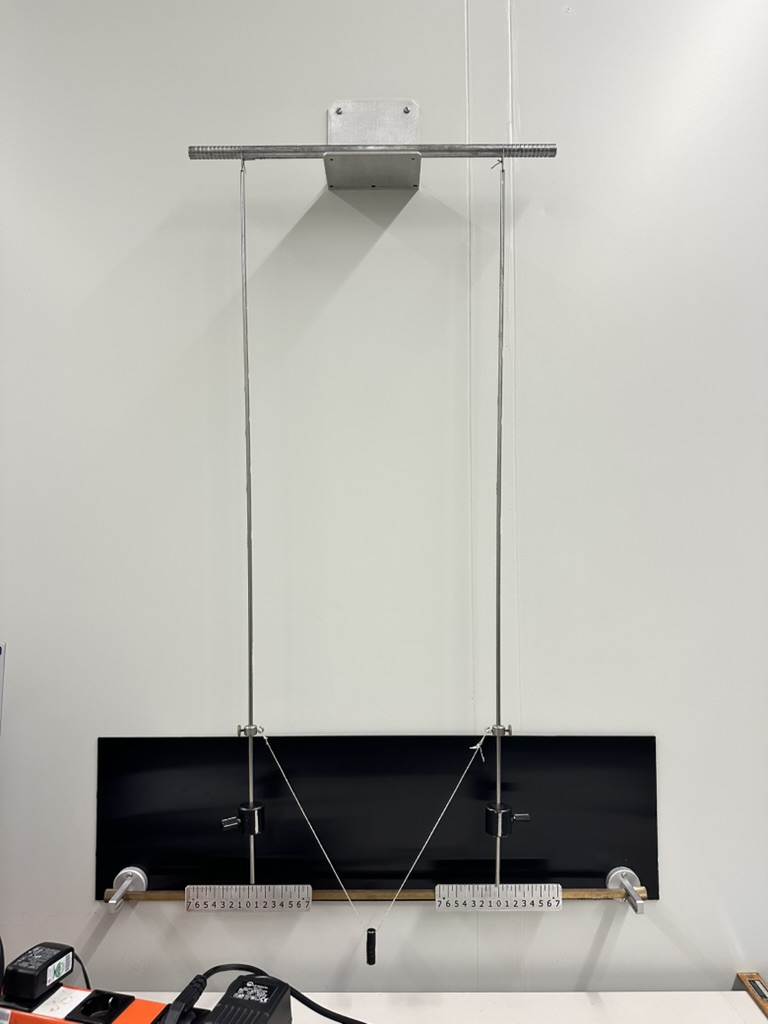
\includegraphics[width=0.4\textwidth]{Aufbau}}
	\caption{Aufbau der Pendel, die hier bei \(\lh = \qty{70}{\centi\meter}\) gekoppelt sind.}
	\label{fig:aufbau}
\end{figure}

Die Pendel werden durch lange, dünne Metallstäbe realisiert, die durch eine Fadenöse auf einem horizontal befestigten Metallstab gelagert sind, und auf deren Enden Massen gezogen und dann mit einer Schraube festgezogen werden können. Nach demselben Prinzip werden die Haken als Aufnahmepunkte für die Verbindung zwischen beiden Pendeln über den Massen installiert. Um die Pendel zu koppeln wird eine Schnur, die durch eine weitere Masse führt in die Haken eingehängt.

Von einer CCD-Kamera wird die Momentanauslenkung der Massen aufgezeichnet. Dafür sind an den Massen vertikal reflektierende Streifen angebracht. Der Fokus der Kamera wird auf \qty{0,9}{\meter} eingestellt. Die Blende wurde auf \num{11} eingestellt.

Mit einer Metallleiste, an der zwei verschiebbare Stopper angebracht sind, lassen sich die Pendel bestmöglich gleichphasig mit gleicher Amplitude auslenken. Um die gegensinnige Fundamentalschwingung zu erzeugen kann auch das Kopplungsgewicht nach unten gezogen werden.

Um die relevanten Daten zur Periodendauerbestimmung eines Pendels zu erhalten wird wie folgt vorgegangen: Nach einer initialen Auslenkung wird im Messprogramm die Aufzeichnung gestartet und nach ca. \qty{60}{\second} gestoppt. Dann wird ein Extremum der Auslenkung zu Beginn der Aufzeichnung ausgewählt, der zugehörige Zeitpunkt notiert, \num{20} Perioden abgezählt und wieder der Zeitpunkt notiert, um daraus die Differenz zu bilden. Wird der Schwebungsfall gemessen, werden mindestens \num{5} Minima abgewartet. Dann wird die Aufzeichnung beendet und der Zeitpunkt des ersten Stillstandes notiert. Beim vierten Stillstand des Pendels wird dieser Zeitpunkt vermerkt.

\section{Messwerte}

\begin{table}[H]
		\caption{Massen und Längen der zwei Pendel \label{tbl:dimensions}}
	\begin{tabular*}{\textwidth}{@{\extracolsep{\fill}}@{\hspace{5pt}}lrr@{\hspace{5pt}}}
		\toprule
		Parameter & Pendel \num{1} & Pendel \num{2}\\
		\midrule
		\(m\) in \si{\kilogram} & \num{176,97e-3}   & \num{174,95e-3}\\
		\(m_{\text{H}}\) in \si{\kilogram} & \num{16,06e-3}   & \num{15,80e-3}\\
		\(m_{\text{St}}\) in \si{\kilogram} & \num{131,40e-3} & \num{131,27e-3}\\
		\(L\) in \si{\meter} & \num{0,804} & \num{0,800}\\
		\(\lh\) in \si{\meter} & \num{0,4} & \num{0,4}\\
		\(L_{\text{St}}\) in \si{\meter} & \num{0,87} & \num{0,87}\\
		\bottomrule
	\end{tabular*}
\end{table}

\(t_0\) und \(t_1\) stehen im ungekoppelten Fall, sowie im gekoppelten Fall für die Fundamentalschwingungen stets für Zeitpunkte, zwischen denen \num{20} Perioden durchlaufen wurden. Im Schwebungsfall sind mit \(t_i\) alle Zeiten vermerkt, zu der das Pendel stillsteht.

\newpage

Im Folgenden sind die Messwerte für die Position \(\lh = \qty{40}{\centi\meter}\) tabelliert.

\begin{table}[H]
		\caption{Ungekoppelter gleichsinniger Fall \label{tbl:ngekgl40}}
	\begin{tabular*}{\textwidth}{@{\extracolsep{\fill}}@{\hspace{5pt}}lrr@{\hspace{5pt}}}
		\toprule
		Pendel & \(t_0\) in \(\si{\second}\) & \(t_1\) in \(\si{\second}\)\\
		\midrule
		1 & \num{1,4}   & \num{35,5}\\
		2 & \num{1,3}   & \num{35,4}\\
		\bottomrule
	\end{tabular*}
\end{table}

\begin{table}[H]
		\caption{Gekoppelter gleichsinniger Fall \label{tbl:gekgl40}}
	\begin{tabular*}{\textwidth}{@{\extracolsep{\fill}}@{\hspace{5pt}}lrr@{\hspace{5pt}}}
		\toprule
		Pendel & \(t_0\) in \(\si{\second}\) & \(t_1\) in \(\si{\second}\)\\
		\midrule
		1 & \num{0,9}   & \num{34,8}\\
		2 & \num{0,8}   & \num{34,8}\\
		\bottomrule
	\end{tabular*}
\end{table}

\begin{table}[H]
		\caption{Gekoppelter gegensinniger Fall \label{tbl:gekgeg40}}
	\begin{tabular*}{\textwidth}{@{\extracolsep{\fill}}@{\hspace{5pt}}lrr@{\hspace{5pt}}}
		\toprule
		Pendel & \(t_0\) in \(\si{\second}\) & \(t_1\) in \(\si{\second}\)\\
		\midrule
		1 & \num{0,4}   & \num{33,3}\\
		2 & \num{1,2}   & \num{34,1}\\
		\bottomrule
	\end{tabular*}
\end{table}

\begin{table}[H]
		\caption{Schwebungsfall \label{tbl:schweb40}}
	\begin{tabular*}{\textwidth}{@{\extracolsep{\fill}}@{\hspace{5pt}}lrrrrr@{\hspace{5pt}}}
		\toprule
		Pendel & \(t_0\) in \(\si{\second}\) & \(t_1\) in \(\si{\second}\)& \(t_2\) in \(\si{\second}\)& \(t_3\) in \(\si{\second}\)& \(t_4\) in \(\si{\second}\)\\
		\midrule
		1 & \num{0,0}   & \num{52,4} & \num{105,8} & \num{160,0} & \num{211,6}\\
		2 & \num{25,4}   & \num{79,5} & \num{132,9} & \num{185,3} & \num{237,8}\\
		\bottomrule
	\end{tabular*}
\end{table}

\newpage

Im Folgenden sind die Messwerte für die Position \(\lh = \qty{55}{\centi\meter}\) tabelliert.

\begin{table}[H]
		\caption{Ungekoppelter gleichsinniger Fall \label{tbl:ngekgl55}}
	\begin{tabular*}{\textwidth}{@{\extracolsep{\fill}}@{\hspace{5pt}}lrr@{\hspace{5pt}}}
		\toprule
		Pendel & \(t_0\) in \(\si{\second}\) & \(t_1\) in \(\si{\second}\)\\
		\midrule
		1 & \num{0,8}   & \num{35,0}\\
		2 & \num{0,8}   & \num{34,8}\\
		\bottomrule
	\end{tabular*}
\end{table}

\begin{table}[H]
		\caption{Gekoppelter gleichsinniger Fall \label{tbl:gekgl55}}
	\begin{tabular*}{\textwidth}{@{\extracolsep{\fill}}@{\hspace{5pt}}lrr@{\hspace{5pt}}}
		\toprule
		Pendel & \(t_0\) in \(\si{\second}\) & \(t_1\) in \(\si{\second}\)\\
		\midrule
		1 & \num{0,5}   & \num{34,5}\\
		2 & \num{0,5}   & \num{34,5}\\
		\bottomrule
	\end{tabular*}
\end{table}

\begin{table}[H]
		\caption{Gekoppelter gegensinniger Fall \label{tbl:gekgeg55}}
	\begin{tabular*}{\textwidth}{@{\extracolsep{\fill}}@{\hspace{5pt}}lrr@{\hspace{5pt}}}
		\toprule
		Pendel & \(t_0\) in \(\si{\second}\) & \(t_1\) in \(\si{\second}\)\\
		\midrule
		1 & \num{1,4}   & \num{33,6}\\
		2 & \num{0,6}   & \num{32,9}\\
		\bottomrule
	\end{tabular*}
\end{table}

\begin{table}[H]
		\caption{Schwebungsfall \label{tbl:schweb55}}
	\begin{tabular*}{\textwidth}{@{\extracolsep{\fill}}@{\hspace{5pt}}lrrrrr@{\hspace{5pt}}}
		\toprule
		Pendel & \(t_0\) in \(\si{\second}\) & \(t_1\) in \(\si{\second}\)& \(t_2\) in \(\si{\second}\)& \(t_3\) in \(\si{\second}\)& \(t_4\) in \(\si{\second}\)\\
		\midrule
		1 & \num{14,8}   & \num{44,9} & \num{74,6} & \num{105,2} & \num{134,8}\\
		2 & \num{0,0}   & \num{29,5} & \num{60,2} & \num{89,8} & \num{119,6}\\
		\bottomrule
	\end{tabular*}
\end{table}

\newpage

Im Folgenden sind die Messwerte für die Position \(\lh = \qty{70}{\centi\meter}\) tabelliert.

\begin{table}[H]
		\caption{Ungekoppelter gleichsinniger Fall \label{tbl:ngekgl70}}
	\begin{tabular*}{\textwidth}{@{\extracolsep{\fill}}@{\hspace{5pt}}lrr@{\hspace{5pt}}}
		\toprule
		Pendel & \(t_0\) in \(\si{\second}\) & \(t_1\) in \(\si{\second}\)\\
		\midrule
		1 & \num{1,5}   & \num{35,8}\\
		2 & \num{1,5}   & \num{35,7}\\
		\bottomrule
	\end{tabular*}
\end{table}

\begin{table}[H]
		\caption{Gekoppelter gleichsinniger Fall \label{tbl:gekgl70}}
	\begin{tabular*}{\textwidth}{@{\extracolsep{\fill}}@{\hspace{5pt}}lrr@{\hspace{5pt}}}
		\toprule
		Pendel & \(t_0\) in \(\si{\second}\) & \(t_1\) in \(\si{\second}\)\\
		\midrule
		1 & \num{0,5}   & \num{34,7}\\
		2 & \num{0,5}   & \num{34,7}\\
		\bottomrule
	\end{tabular*}
\end{table}

\begin{table}[H]
		\caption{Gekoppelter gegensinniger Fall \label{tbl:gekgeg70}}
	\begin{tabular*}{\textwidth}{@{\extracolsep{\fill}}@{\hspace{5pt}}lrr@{\hspace{5pt}}}
		\toprule
		Pendel & \(t_0\) in \(\si{\second}\) & \(t_1\) in \(\si{\second}\)\\
		\midrule
		1 & \num{1,5}   & \num{33,0}\\
		2 & \num{0,7}   & \num{32,2}\\
		\bottomrule
	\end{tabular*}
\end{table}

\begin{table}[H]
		\caption{Schwebungsfall \label{tbl:schweb70}}
	\begin{tabular*}{\textwidth}{@{\extracolsep{\fill}}@{\hspace{5pt}}lrrrrr@{\hspace{5pt}}}
		\toprule
		Pendel & \(t_0\) in \(\si{\second}\) & \(t_1\) in \(\si{\second}\)& \(t_2\) in \(\si{\second}\)& \(t_3\) in \(\si{\second}\)& \(t_4\)\(\si{\second}\)\\
		\midrule
		1 & \num{0,0}   & \num{18,1} & \num{38,7} & \num{58,3} & \num{77,8}\\
		2 & \num{9,0}   & \num{29,5} & \num{49,0} & \num{68,6} & \num{88,3}\\
		\bottomrule
	\end{tabular*}
\end{table}

\begin{table}[H]
		\caption{Schwebungsfall für unterschiedlich ausgelenkte Massen \label{tbl:schwebX70}}
	\begin{tabular*}{\textwidth}{@{\extracolsep{\fill}}@{\hspace{5pt}}lrrrrr@{\hspace{5pt}}}
		\toprule
		Pendel & \(t_0\) in \(\si{\second}\) & \(t_1\) in \(\si{\second}\)& \(t_2\) in \(\si{\second}\)& \(t_3\) in \(\si{\second}\)& \(t_4\) in \(\si{\second}\)\\
		\midrule
		1 & \num{6,2}   & \num{26,7} & \num{47,1} & \num{66,9} & \num{85,6}\\
		2 & \num{16,4}   & \num{36,9} & \num{57,3} & \num{77,1} & \num{97,4}\\
		\bottomrule
	\end{tabular*}
\end{table}

\section{Auswertung}

\(T_0\) berechnet sich aus den Daten, die in \autoref{tbl:ngekgl40} eingetragen sind durch
\begin{equation*}
	T_0 = \frac{t_1 - t_0}{20} = \frac{\qty{35,5}{\second} - \qty{1,4}{\second}}{20} = \qty{1,7}{\second} \,.
\end{equation*}
Für Pendel \num{2} folgt analog ebenfalls \(T_0 =\qty{1,7}{\second}\). Somit ist dies auch das Mittel. Dieses Prinzip wird auf alle \(T_{\text{gl}}\) und \(T_{\text{geg}}\) angewendet.

\(T_{\text{II}}\) wird durch \autoref{eq:t2} ermittelt. %Inline Equation Link

Bei \(T_{\text{S}}\) wird der erste und der letzte Zeitpunkt des Stillstandes des Pendel, der in der Messdauer liegt auf die Anzahl der Schwebungsdauern in diesem Intervall normiert. %Wording?!

Für die entsprechenden Kopplungsgrade ergeben sich die folgende Periodendauern.

\begin{table}[H]
		\caption{Periodendauern für \(\lh = \qty{40}{\centi\meter}\) \label{tbl:res40}}
	\begin{tabular*}{\textwidth}{@{\extracolsep{\fill}}@{\hspace{5pt}}lrrr@{\hspace{5pt}}}
		\toprule
		Periodendauer & Pendel 1 & Pendel 2 & Mittel\\
		\midrule
		\(T_{\text{gl}}\) & \qty{1,7}{\second} & \qty{1,7}{\second} & \qty{1,7}{\second}\\
		\(T_{\text{geg}}\) & \qty{1,6}{\second} & \qty{1,6}{\second} & \qty{1,6}{\second}\\
		\(T_{\text{II}}\) & \qty{1,6}{\second} & \qty{1,6}{\second} & \qty{1,6}{\second}\\
		\(T_{\text{S}}\) & \qty{52,9}{\second} & \qty{53,1}{\second} & \qty{53,0}{\second} \\
		\bottomrule
	\end{tabular*}
\end{table}


\begin{table}[H]
		\caption{Periodendauern für \(\lh = \qty{55}{\centi\meter}\) \label{tbl:res55}}
	\begin{tabular*}{\textwidth}{@{\extracolsep{\fill}}@{\hspace{5pt}}lrrr@{\hspace{5pt}}}
		\toprule
		Periodendauer & Pendel 1 & Pendel 2 & Mittel\\
		\midrule
		\(T_{\text{gl}}\) & \qty{1,7}{\second} & \qty{1,7}{\second} & \qty{1,7}{\second}\\
		\(T_{\text{geg}}\) & \qty{1,6}{\second} & \qty{1,6}{\second} & \qty{1,6}{\second}\\
		\(T_{\text{II}}\) & \qty{1,6}{\second} & \qty{1,6}{\second} & \qty{1,6}{\second}\\
		\(T_{\text{S}}\) & \qty{30,0}{\second} & \qty{29,9}{\second} & \qty{30,0}{\second} \\
		\bottomrule
	\end{tabular*}
\end{table}

\begin{table}[H]
		\caption{Periodendauern für \(\lh = \qty{70}{\centi\meter}\) \label{tbl:res70}. \(T_{\text{S},≠}\) sind die Schwebungsdauern die gemessen wurden, als die Schwebung durch ungleiche Auslenkungen erzeugt wurde.}
	\begin{tabular*}{\textwidth}{@{\extracolsep{\fill}}@{\hspace{5pt}}lrrr@{\hspace{5pt}}}
		\toprule
		Periodendauer & Pendel 1 & Pendel 2 & Mittel\\
		\midrule
		\(T_{\text{gl}}\) & \qty{1,7}{\second} & \qty{1,7}{\second} & \qty{1,7}{\second}\\
		\(T_{\text{geg}}\) & \qty{1,6}{\second} & \qty{1,6}{\second} & \qty{1,6}{\second}\\
		\(T_{\text{II}}\) & \qty{1,6}{\second} & \qty{1,6}{\second} & \qty{1,6}{\second}\\
		\(T_{\text{S}}\) & \qty{19,5}{\second} & \qty{19,8}{\second} & \qty{19,6}{\second} \\
		\(T_{\text{S},≠}\) & \qty{19,9}{\second} & \qty{20,3}{\second} & \qty{20,1}{\second}\\
		\bottomrule
	\end{tabular*}
\end{table}

Die folgende Abbildung zeigt eine gleichsinnige Fundamentalschwingung über einige Perioden. Wie zu sehen ist, wird sie dadurch charakterisiert, dass es annähernd keine Phasenverschiebung gibt und die Amplituden gleich sind.
\begin{figure}[H]
	\centering{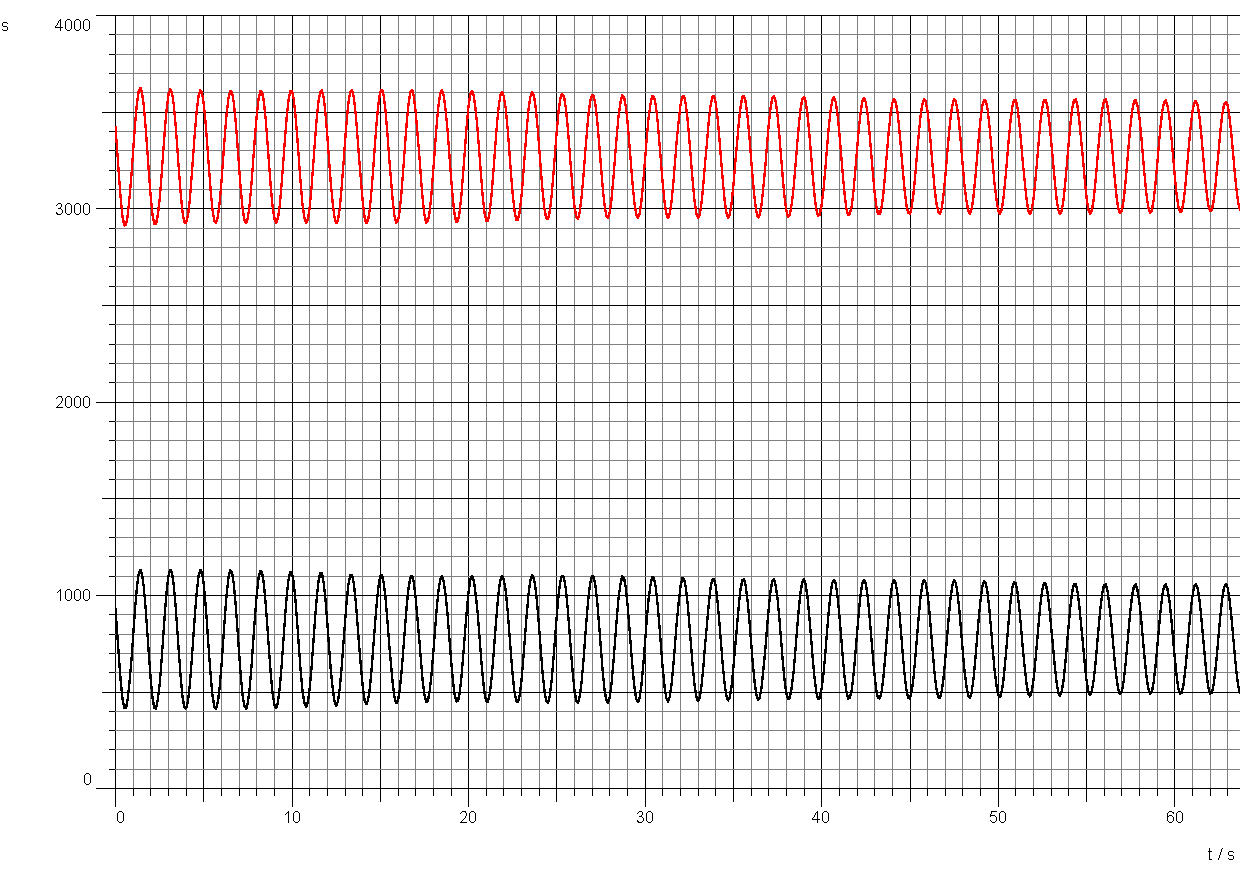
\includegraphics[width=0.7\textwidth]{gleichsinnige_FUNDAMENTALSCHWINGUNG_70cm.pdf}}
	\caption{\(s(t)\)-Diagramm der gleichsinnigen Fundamentalschwingung bei \(\lh = \qty{70}{\centi\meter}\).}
	\label{fig:gl70}
\end{figure}

Die folgende Abbildung zeigt eine gegensinnige Fundamentalschwingung über einige Perioden. Sie zeichnet sich durch eine Phasenverschiebung von \(\frac{\pi}{2}\) aus. Ihre Amplituden sind ebenfalls gleich.
\begin{figure}[H]
	\centering{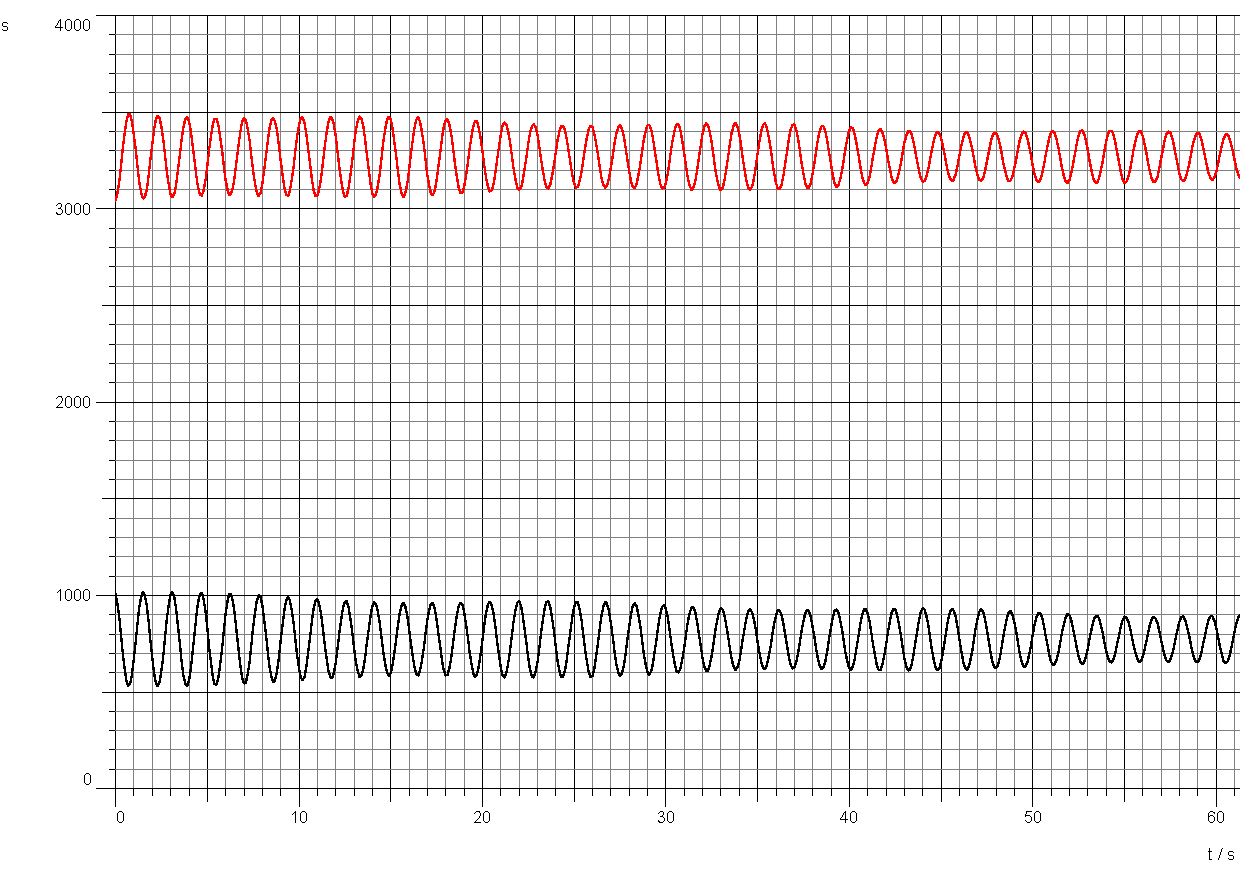
\includegraphics[width=0.7\textwidth]{gegensinnige_FUNDAMENTALSCHWINGUNG_70cm.pdf}}
	\caption{\(s(t)\)-Diagramm der gegensinnigen Fundamentalschwingung bei \(\lh = \qty{70}{\centi\meter}\).}
	\label{fig:geg70}
\end{figure}

Wird der Schwebungsfall durch auslenken eines Pendels herbigeführt entsteht folgendes Schwingungsmuster, wobei die Schwebungsdauern gut sichtbar werden.
\begin{figure}[H]
	\centering{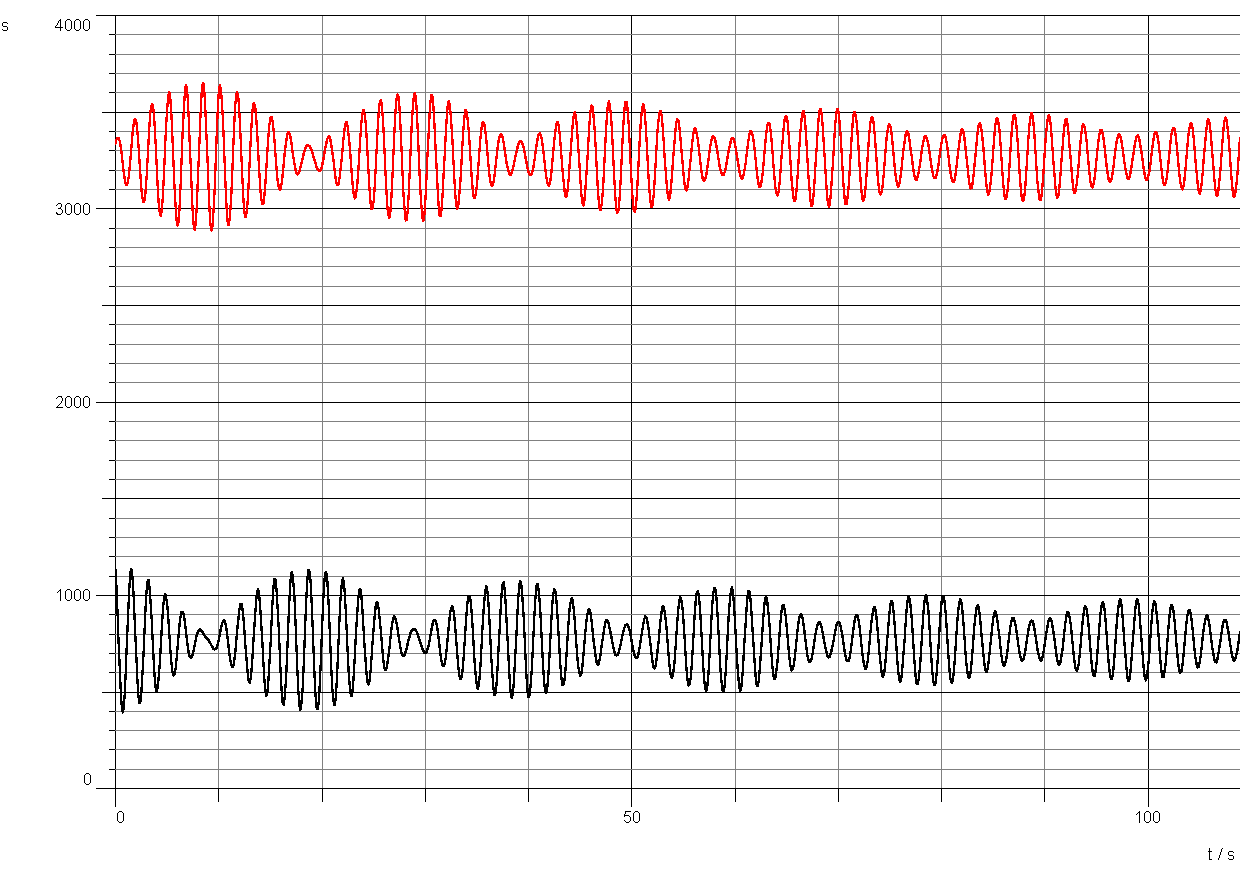
\includegraphics[width=0.7\textwidth]{SCHWEBUNG_70cm.pdf}}
	\caption{\(s(t)\)-Diagramm des Schwebungsfalles bei \(\lh = \qty{70}{\centi\meter}\).}
	\label{fig:schweb}
\end{figure}

Der Schwebungsfall ensteht ebenfalls, wenn man beide Pendel ungleich auslenkt. Dann lassen sich folgende Schwingungen beobachten.
\begin{figure}[H]
	\centering{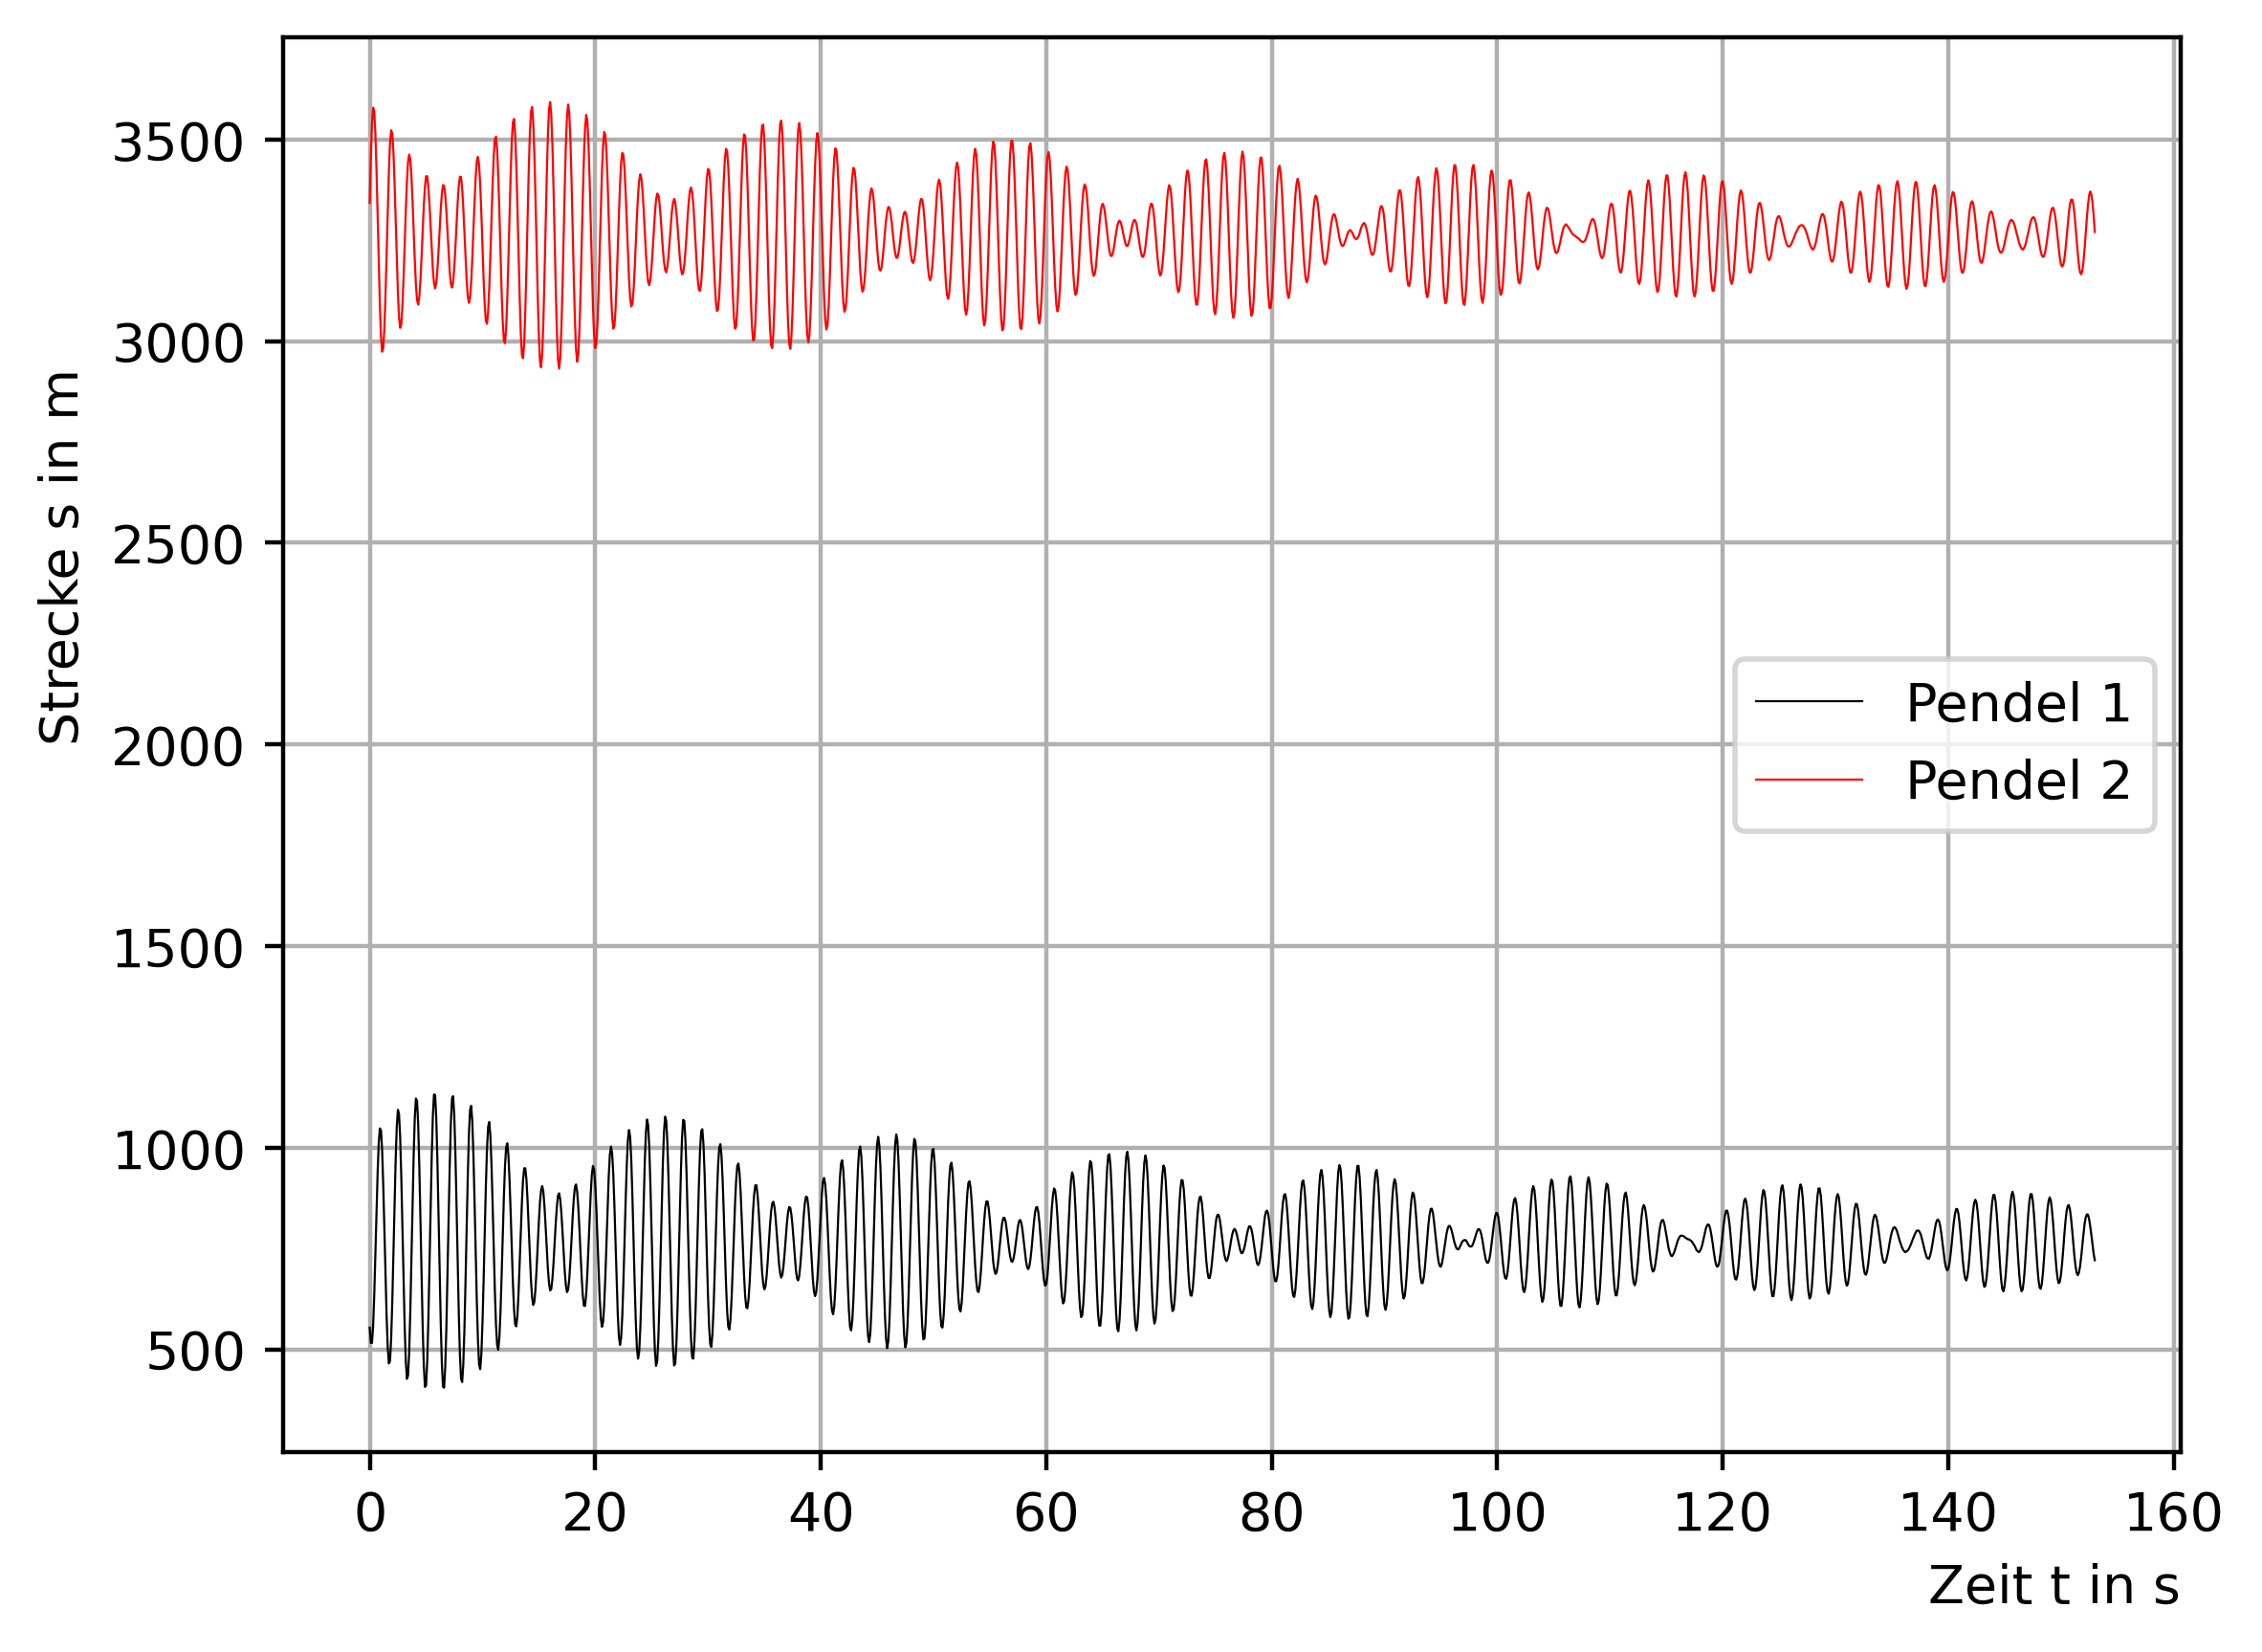
\includegraphics[width=0.75\textwidth]{ungleicherSchweb.png}}
	\caption{\(s(t)\)-Diagramm des Schwebungsfalles bei \(\lh = \qty{70}{\centi\meter}\) und ungleich ausgelenkten Pendeln.}
	\label{fig:ungl70}
\end{figure}

Wie aus \autoref{tbl:res70} hervorgeht, liegen \(T_{\text{S}}\) und \(T_{\text{S},≠}\) sehr nah beieinander. Daran lässt sich sehen, dass die Schwebungsdauer nicht davon abhängt, ob nur ein Pendel oder beide ausgelenkt werden. Bei letztem Schwingungsmode ist zu beachten, dass die Auslenkungen ungleich sein müssen, das sonst wieder Fundamentalschwingungen entstehen würden. Dies liegt daran, dass die Schwebungsdauer nur von den Eigenfrequenzen des Systems abhängt, und diese ändern sich nicht, solange man die Dimensionen des Systems nicht manipuliert bzw. den Kopplungsgrad nicht verändert.

%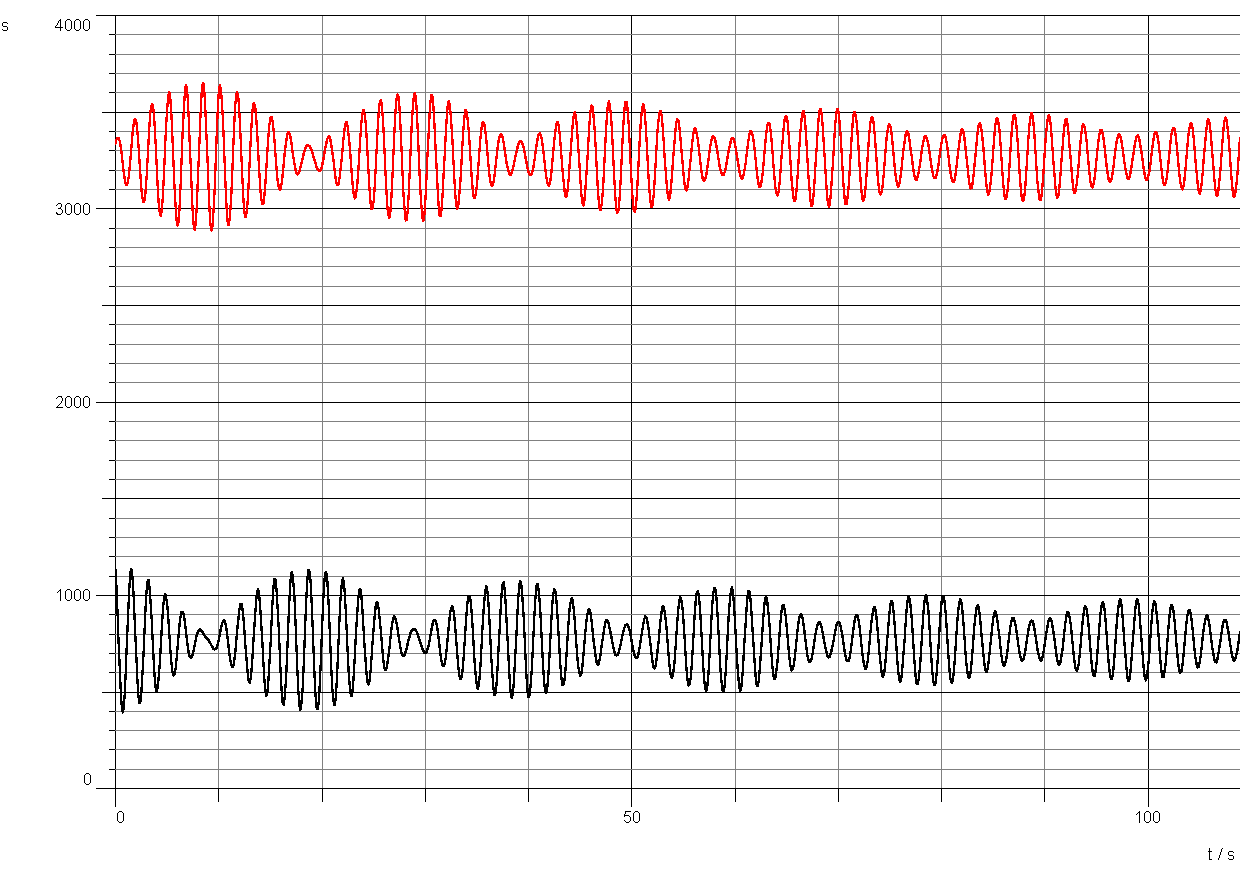
\includepdf[pages=-]{SCHWEBUNG_70cm.pdf}
%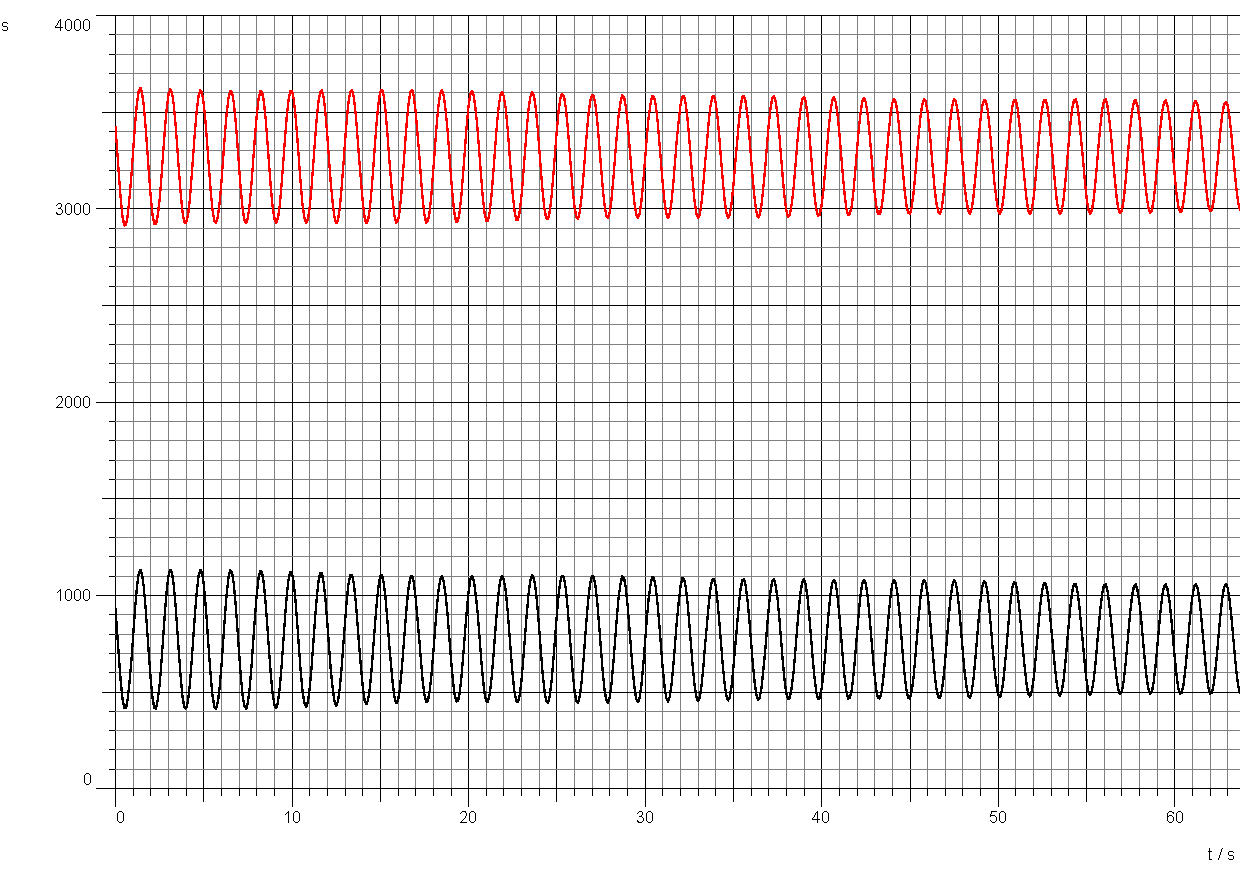
\includepdf[pages=-]{gleichsinnige_FUNDAMENTALSCHWINGUNG_70cm.pdf}
%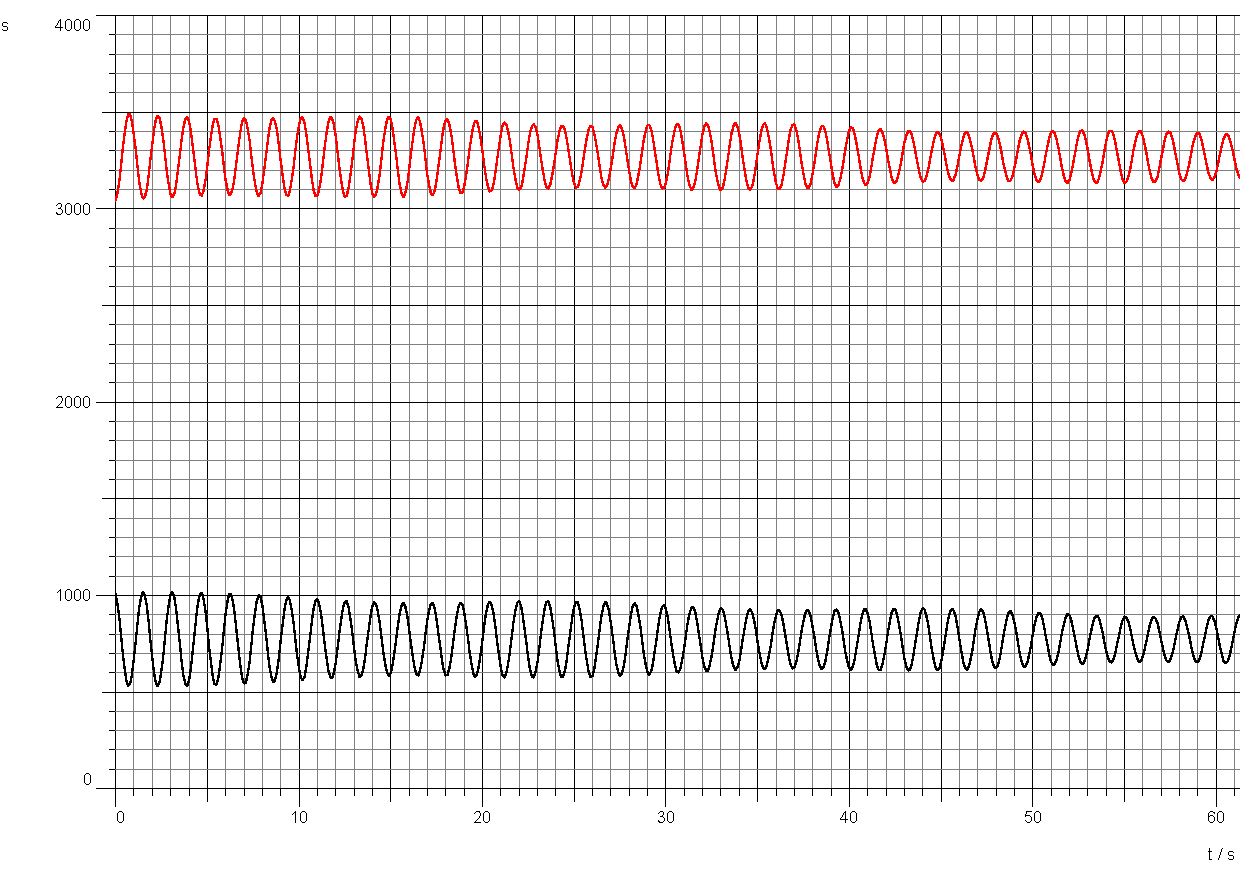
\includepdf[pages=-]{gegensinnige_FUNDAMENTALSCHWINGUNG_70cm.pdf}

Nach \autoref{eq:trägheitsmom} wird das Gesamtträgheitsmoment mit den Daten aus \autoref{tbl:dimensions} berechnet. Für das erste Pendel ergibt sich das Trägheitsmoment
\begin{equation*}
	\begin{split}
		J_1 = \frac{1}{3} \cdot \qty{131,40e-3}{\kilogram} \cdot (\qty{0,87}{\meter})^2 &+ \qty{16,06e-3}{\kilogram} \cdot (\qty{0,4}{\meter})^2
		\\&+ \qty{176,97e-3}{\kilogram} \cdot (\qty{0,804}{\meter})^2 = \qty{0,150}{\kilogram\meter\squared}
	\end{split}
\end{equation*}
und für das zweite Pendel \(J_2 = \qty{0,148}{\kilogram\meter\squared}\).

Die Eigenfrequenz \(\omega_0\) wird mittels \autoref{eq:eig} %Der Link ist komisch
berechnet. Dafür muss zuerst die Lage des Schwerpunktes \(\ls\) mit \autoref{eq:schwerp} berechnet werden und ergibt
\begin{equation}
	\ls = \frac{Lm + \lh m_{\text{H}} + \tfrac{1}{2} \cdot L_{\text{St}} m_{\text{St}}}{m + m_{\text{H}} + m_{\text{St}}}
\end{equation}
\begin{equation*}
	\begin{split}
		\ell_{\text{S},1} &= (\qty{0,804}{\meter} \cdot \qty{176,97e-3}{\kilogram} + \qty{0,4}{\meter} \cdot \qty{16,06e-3}{\kilogram}\\
		&+ \tfrac{1}{2} \cdot \qty{0,87}{\meter} \cdot \qty{131,40e-3}{\kilogram})\\
		&\cdot \mleft(\mleft(\num{176,97e-3} + \num{16,06e-3} + \num{131,40e-3}\mright)\si{\kilogram}\mright)^{-1}\\
		&= \qty{0,635}{\meter} \,.
	\end{split}
\end{equation*}
Für \(\ell_{\text{S},2}\) ergibt sich \(\ell_{\text{S},2} = \qty{0,632}{m}\). Die Schwerpunktmasse des ersten Pendels \(M_1\) ist
\begin{equation*}
	\begin{split}
		M_1 &= m_1 + m_{\text{H},1} + m_{\text{St},1}\\
		&= \qty{176,97e-3}{\kilogram} + \qty{16,06e-3}{\kilogram} + \qty{131,40e-3}{\kilogram}\\
		&= \qty{324,43e-3}{\kilogram} \,.
	\end{split}
\end{equation*}
Für das zweite Pendel ist \(M_2 = \qty{322,02e-3}{\kilogram}\). Damit beläuft sich die theoretische Eigenfrequenz \(\omega_{0,1,\text{theo}}\) auf
\begin{equation*}
	\omega_{0,1,\text{theo}} = \sqrt{\frac{M_1 g \ls}{J_1}} = \sqrt{\frac{\qty{324,43e-3}{\kilogram} \cdot \qty{9,81}{\meter\per\second\squared} \cdot \qty{0,635}{\meter}}{\qty{0,150}{\kilogram\meter\squared}}} = \qty{3,671}{\hertz}.
\end{equation*}
Folgerichtig gilt \(\omega_{0,2,\text{theo}} = \qty{3,673}{\hertz}\).

Aus den gemessenen Größen ergeben sich die gemessenen Eigenfrequenzen
\begin{equation*}
	\omega_{0,1,\text{mess}} = \frac{2\pi}{\qty{1,7}{\second}} = \qty{3,7}{\hertz}
\end{equation*}
und \(\omega_{0,2,\text{mess}} = \qty{3,7}{\hertz}\).

Für \(\lh = \qty{40}{\centi \meter}\) lässt sich der Kopplungsgrad nach \autoref{eq:2} berechnen durch
\begin{align*}
	K_1 &= \frac{(\qty{1,7}{\second})^2 - (\qty{1,6}{\second})^2}{(\qty{1,7}{\second})^2 + (\qty{1,6}{\second})^2}\\
	&= \num{0,0606}
\end{align*}
und mittels \autoref{eq:3} durch
\begin{align*}
	K_2 &= 4 \cdot \frac{\qty{52,9}{\second} \cdot \qty{1,6}{\second}}{4 \cdot (\qty{52,9}{\second})^2 + (\qty{1,6}{\second})^2}\\
	&= \num{0,0302}
\end{align*}

Damit ergeben sich die in \autoref{tbl:kopplungsgrade} dargestellten Kopplungsgrade für die anderen Kopplungsstärken.

\begin{table}[H]
		\caption{Kopllungsgrade berechnet durch verschiedene Gleichungen. \label{tbl:kopplungsgrade}}
	\begin{tabular*}{\textwidth}{@{\extracolsep{\fill}}@{\hspace{5pt}}lrr@{\hspace{5pt}}}
		\toprule
		Länge \(\lh\) in \si{\centi\meter} & \(K_1\) nach \autoref{eq:2} & \(K_2\) nach \autoref{eq:3}\\
		\midrule
		\num{40} & \num{0,0606} & \num{0,0302}\\
		\num{55} & \num{0,0606} & \num{0,0533}\\
		\num{70} & \num{0,0606} & \num{0,0815}\\
		\bottomrule
	\end{tabular*}
\end{table}
Die Kopplungsgrade verändern sich nur geringfügig. Dabei sollte \autoref{eq:2} die genaueren Ergebnisse liefern, da er mit den direkt gemessenen Periodendauern berechnet werden kann, während bei \autoref{eq:3} mehrere Messungen und Rechnungen für \(T_{\text{II}}\) nötig sind, wodurch größere Unsicherheiten das Ergebnis verfälschen.

\section{Fehlerrechnung}

Die Messfehler sind gegeben durch
\begin{align*}
	\Delta m &= \qty{0,01e-3}{\kilogram},\\
	\Delta T_{\text{geg}} = \Delta T_{\text{gl}} &= \qty{0,01}{\second},\\
	\Delta T_{\text{S}} &= \qty{0,3}{\second}.
\end{align*}

Fehlerfortpflanzung für das Trägheitsmoment:
\begin{align*}
	\Delta J &= \abs{\pdv{J}{m}} \cdot \Delta m = \Le(\frac{1}{3} \cdot L_{\text{St}}^2 + \lh^2 + L^2\Ri) \cdot \Delta m\\
	&= \qty{1,1e-5}{\kilogram\meter\squared}.
\end{align*}

Fehlerfortpflanzung für die Schwerpunktmasse:
\begin{equation*}
	\Delta M = \abs{\pdv{M}{m}} \cdot \Delta m = \qty{3e-5}{\kilogram}.
\end{equation*}

Fehlerfortpfalnzung für die Frequenz:

Für \(\omega_{0,\text{theo}} = \sqrt{\frac{Mg\ls}{J}}\) gilt:
\begin{align*}
	\Delta \omega_0 &= \abs{\pdv{\omega_0}{M}} \cdot \Delta M + \abs{\pdv{\omega_0}{J}} \cdot \Delta J\\
	&= \frac{1}{2} \Le(\sqrt{\frac{g\ls}{MJ}} \cdot \Delta M + \sqrt{\frac{Mg\ls}{J^3}} \cdot \Delta J\Ri)\\
	&= \qty{12,9e-3}{\hertz}.
\end{align*}
Für \(\omega_{0,\text{mess}} = \frac{2\pi}{T}\) gilt:
\begin{align*}
	\Delta \omega_0 &= \abs{\pdv{\omega_0}{T}} \cdot \Delta T = \frac{2\pi}{T^2} \cdot \Delta T\\
	&= \qty{21,7e-3}{\hertz}.
\end{align*}

Fehlerfortpflanzung für den Kopplungsgrad nach \autoref{eq:2}:
\begin{align*}
	\Delta K_1 &= \abs{\pdv{K_1}{T_{\text{gl}}}} \cdot \Delta T_{\text{gl}} + \abs{\pdv{K_1}{T_{\text{geg}}}} \cdot T_{\text{geg}}\\
	&= 4 \cdot \Delta \tgl \cdot \frac{\tgl\tgeg^2 + \tgeg\tgl^2}{\Le(\tgl^2 + \tgeg^2\Ri)^2}\\
	&=\num{12,1e-3}.
\end{align*}

Fehlerfortpflanzung für den Kopplungsgrad nach \autoref{eq:3}:
\begin{align*}
	\Delta \omz &= \abs{\pdv{\omz}{\omgeg}} \cdot \Delta \omgeg + \abs{\pdv{\omz}{\omgl}} \cdot \Delta \omgl = \frac{1}{2} \cdot \Delta \omgeg + \frac{1}{2} \cdot \Delta \omgl\\
	&= \qty{23,1e-3}{\hertz}.
\end{align*}
\begin{align*}
	\Delta T_{\text{II}} &= \abs{\pdv{T_{\text{II}}}{\omz}} \cdot \Delta \omz = \frac{2\pi}{\omz^2} \cdot \Delta \omz\\
	&= \qty{e-2}{\second}.
\end{align*}
\begin{align*}
	\Delta K_2 &= \abs{\pdv{K_2}{T_{\text{S}}}} \cdot \Delta T_{\text{S}} + \abs{\pdv{K_2}{T_{\text{II}}}} \cdot \Delta T_{\text{II}}\\
	&= 4 \cdot \Le(\frac{4 \tz\ts^2 - \tz^2}{\Le(4\ts^2 + \tz^2\Ri)^2} \cdot \Delta \ts + \frac{4\ts^3 - \ts\tz^2}{\Le(4\ts^2 + \tz^2\Ri)^2} \cdot \Delta \tz\Ri).
\end{align*}

\begin{table}[H]
		\caption{Fehler des Kopplungsgrads \(K_2\) bei verschiedenen Kopplungen. \label{tbl:FehlerK}}
	\begin{tabular*}{\textwidth}{@{\extracolsep{\fill}}@{\hspace{5pt}}lr@{\hspace{5pt}}}
		\toprule
		Länge \(\lh\) in \si{\centi\meter} & \(\Delta K_2\)\\
		\midrule
		\num{40} & \num{0,2e-3}\\
		\num{55} & \num{0,5e-3}\\
		\num{70} & \num{1,3e-3}\\
		\bottomrule
	\end{tabular*}
\end{table}

\section{Zusammenfassung}

Die Trägheitsmomente bei der Koppelposition \(\lh = \qty{40}{\centi\meter}\) wurden berechnet zu \(J_1 = \qty{150(0,011)}{\gram\meter\squared}\) für das erste Pendel und \(J_2 = \qty{148(0,011)}{\gram\meter\squared}\). Damit ergaben sich die berechneten Eigenfrequenzen \(\omega_{0,1,\text{theo}} = \qty{3,671(0,0129)}{\hertz}\) und \(\omega_{0,2,\text{theo}} = \qty{3,673(0,0129)}{\hertz}\). Die gemessenen Eigenfrequenzen wurden auf \(\omega_{0,1,\text{mess}} = \omega_{0,2,\text{mess}} = \qty{3,7(0,0217)}{\hertz}\). Somit stimmen die theoretischen und gemessenen Eigenfrequenzen innerhalb der Fehlergrenze überein.

Mit \autoref{eq:2} wurde der Kopplungsgrad bei jeder Kopplungsposition auf \(K = \num{0,0606(0,0121)}\) bestimmt. Mit \autoref{eq:3} wurde der Kopplungsgrad bei \(\lh = \qty{40}{\centi\meter}\) auf \num{0,0302(0,0002)}, bei \(\lh = \qty{55}{\centi\meter}\) auf \num{0,0533(0,0005)} und bei \(\lh = \qty{70}{\centi\meter}\) auf \num{0,0815(0,0013)} bestimmt.

\begin{thebibliography}{999}
	\bibitem{Quelle} Versuchsanleitung zu \emph{M23 -- Gekoppelte Pendel} (Abgerufen am 25.09.2025).
	Online verfügbar unter: \url{https://www3.physik.uni-stuttgart.de/studium/praktika/ap/pdf_dateien/M23.pdf}
\end{thebibliography}

%\printbibliography
\section{Anhang}

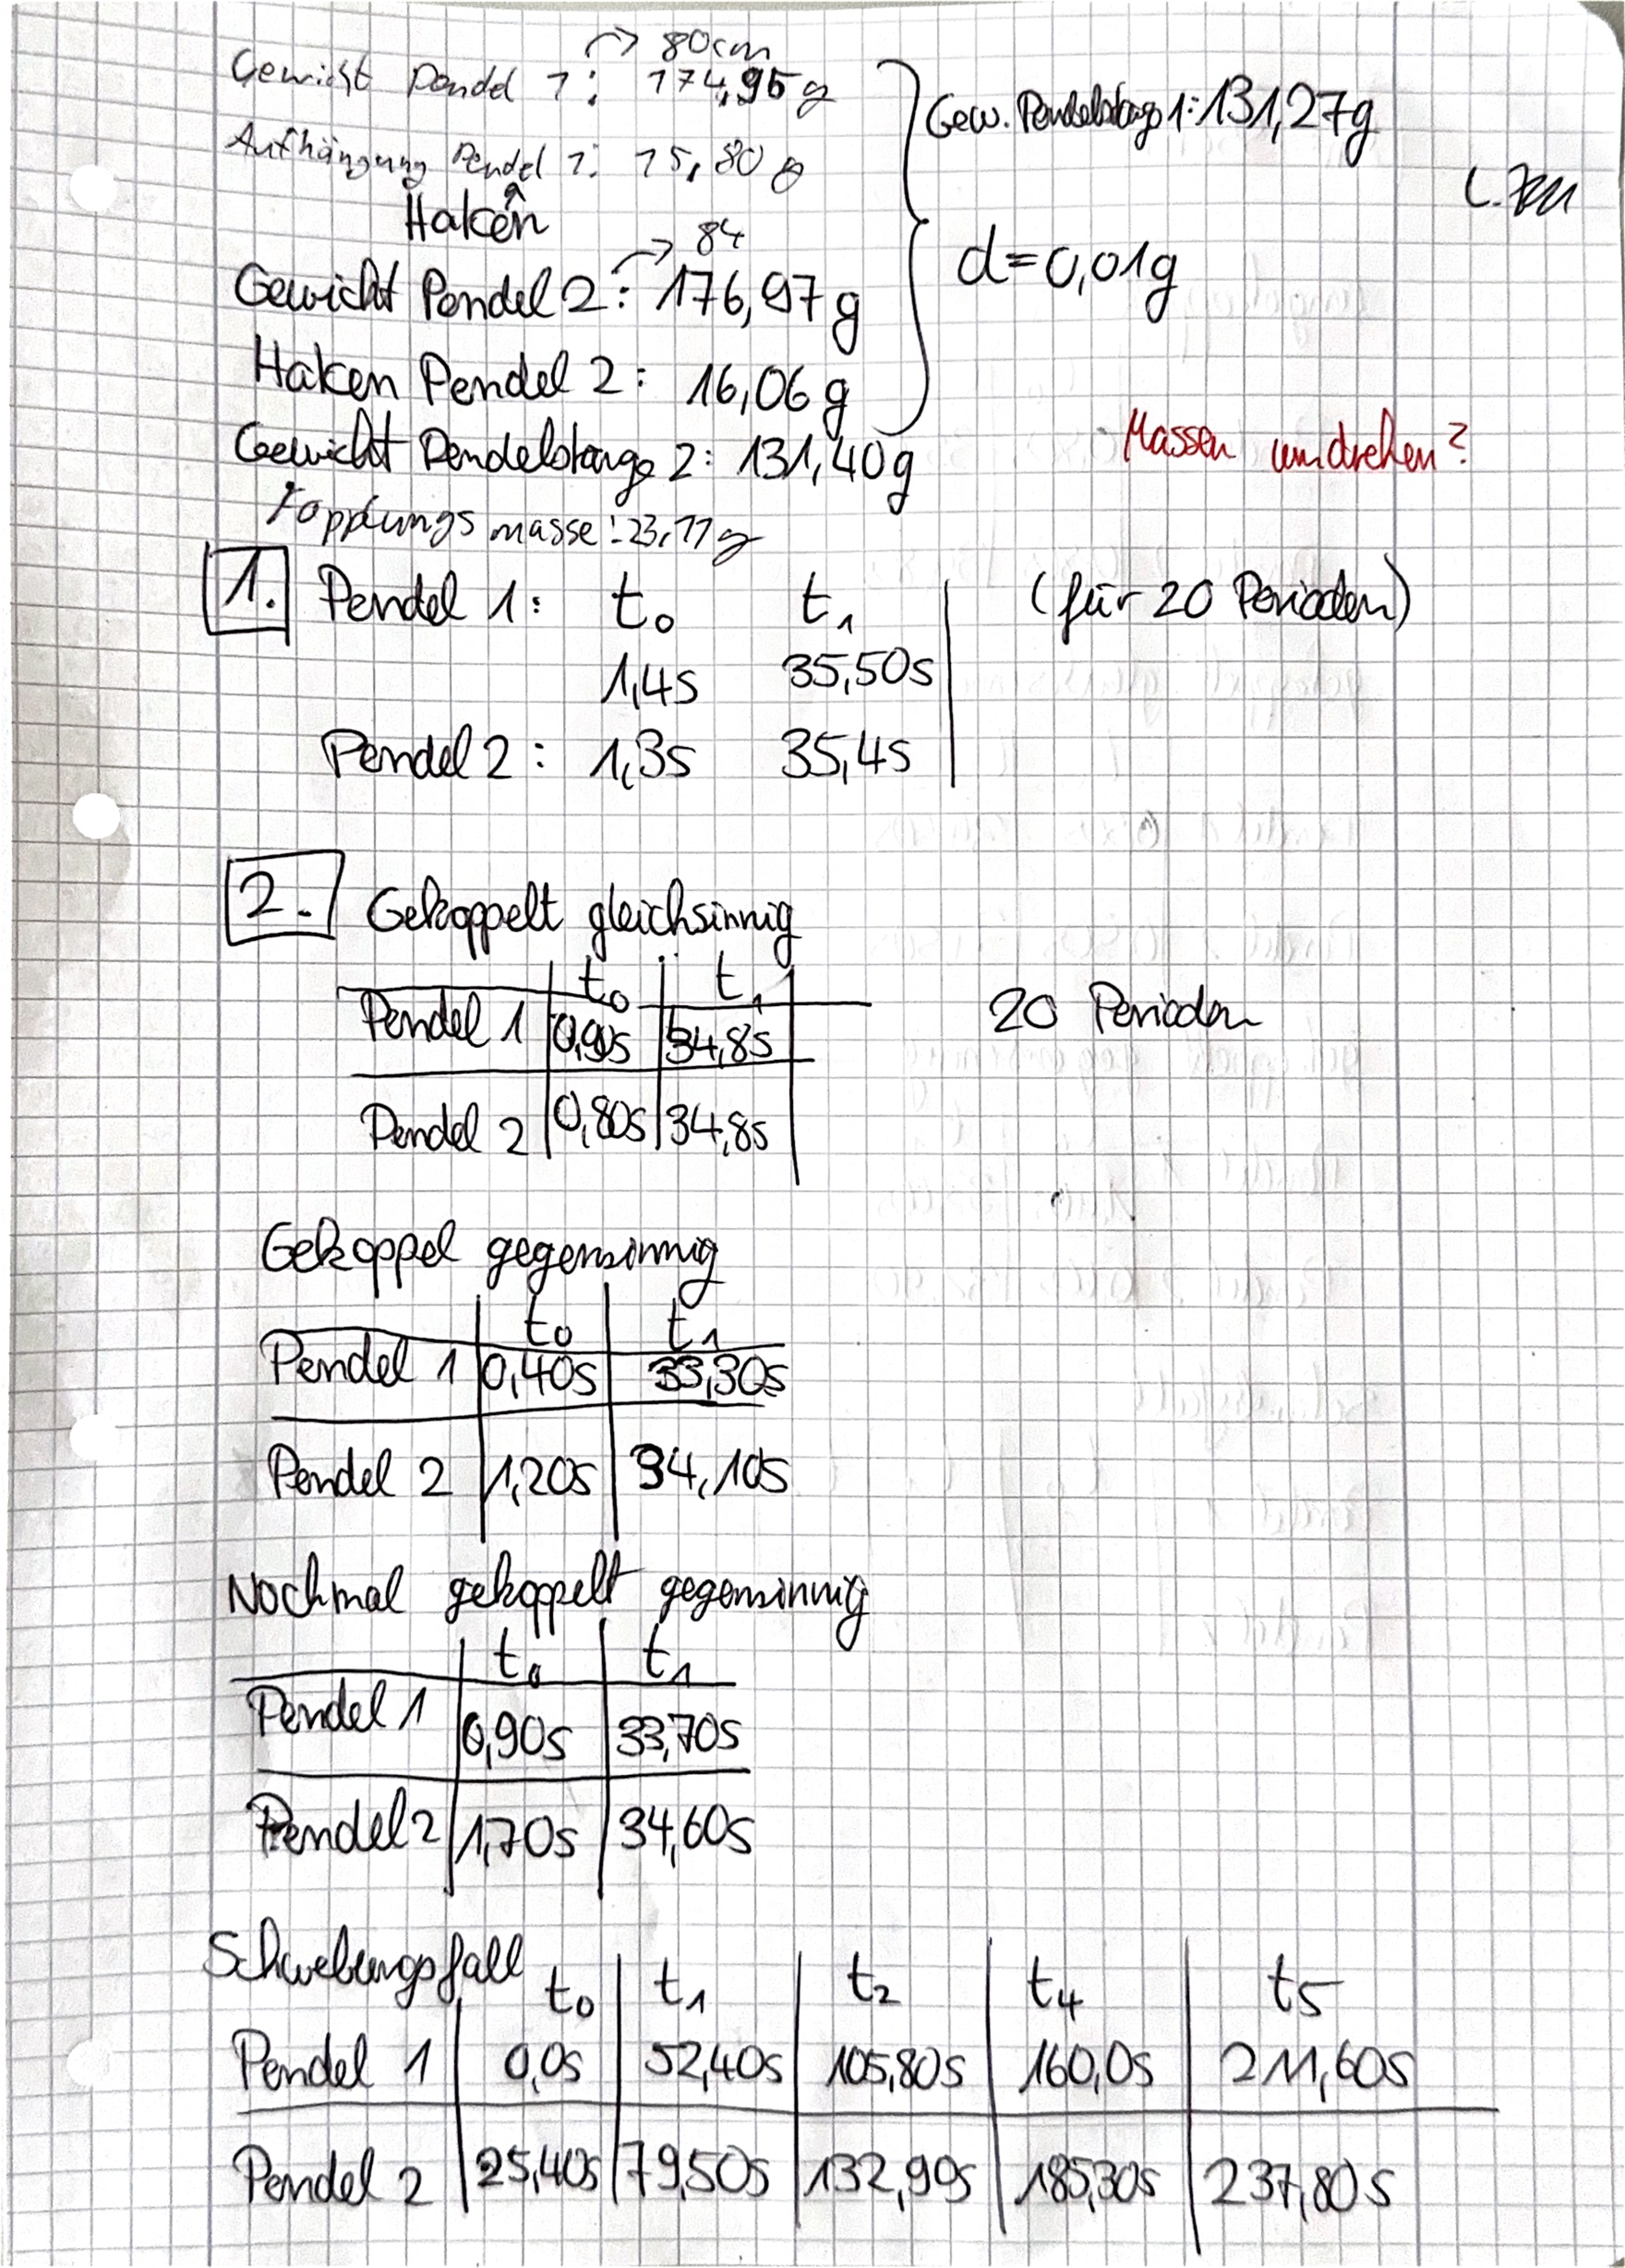
\includepdf[pages=-]{Messprotokoll.pdf}

\end{document}